\documentclass[aspectratio=169]{beamer}

\resetcounteronoverlays{exx}
\usepackage[utf8]{inputenc}
\usepackage[backend=biber, style=authoryear-icomp]{biblatex}
\usepackage{tikz}
\usepackage{blindtext}
\usepackage{tipa}
\usepackage{cgloss4e}
\usepackage{gb4e}
\usepackage{qtree}
\usepackage{enumerate}
\usepackage{longtable}
\usepackage{textgreek}
\usepackage{parskip}
\usepackage{color}
\usepackage{textcomp}
\addbibresource{$HOME/Documents/LaTeX/uni.bib}

\newcommand{\normalgame}{
\begin{figure}
\begin{center}
\tikzstyle{level 1}=[level distance=1.5cm, sibling distance=6.5cm]
\tikzstyle{level 2}=[level distance=1.5cm, sibling distance=3cm]
\tikzstyle{level 3}=[level distance=1.5cm, sibling distance=1.75cm]
\tikzstyle{level 4}=[level distance=1.5cm, sibling distance=2cm]
\begin{tikzpicture}
\node {Nature}
	child{
		node{Speaker}
		child{
			node(d){Hearer}
			child{
				node{$\displaystyle\binom{c}{c}$}
				edge from parent
				node[left]{$S$}
			}
			child{
				node{$\displaystyle\binom{-i}{-i}$}
				edge from parent
				node[right]{$I$}
			}
		edge from parent
		node[left]{$A$}
		}
		child{
			node(a){Hearer}
			child{
				node{$\displaystyle\binom{-p}{0}$}
				edge from parent
				node[left]{$S$}
			}
			child{
				node{$\displaystyle\binom{c-p-i}{c-i}$}
				edge from parent
				node[right]{$I$}
			}
		edge from parent
		node[right]{$P$}
		}
	edge from parent
	node[left]{${Sub}>{Obj}$}
	}
	child{
		node{Speaker}
		child{
			node(b){Hearer}
			child{
				node{$\displaystyle\binom{0}{0}$}
				edge from parent
				node[left]{$S$}
			}
			child{
				node{$\displaystyle\binom{c-i}{c-i}$}
				edge from parent
				node[right]{$I$}
			}
		edge from parent
		node[left]{$A$}
		}
		child{
			node(c){Hearer}
			child{
				node{$\displaystyle\binom{c-p}{c}$}
				edge from parent
				node[left]{$S$}
			}
			child{
				node{$\displaystyle\binom{-p-i}{-i}$}
				edge from parent
				node[right]{$I$}
			}
		edge from parent
		node[right]{$P$}
		}
	edge from parent
	node[right]{${Obj}>{Sub}$}
	};
\draw [dashed](d)to[in=180](b);
\draw [dashed](a)to[in=180](c);
\end{tikzpicture}
\end{center}
\end{figure}}

\newcommand{\scramblegame}{
\begin{figure}
\begin{center}
\tikzstyle{level 1}=[level distance=1.5cm, sibling distance=6.5cm]
\tikzstyle{level 2}=[level distance=1.5cm, sibling distance=3cm]
\tikzstyle{level 3}=[level distance=1.5cm, sibling distance=1.75cm]
\tikzstyle{level 4}=[level distance=1.5cm, sibling distance=2cm]
\begin{tikzpicture}
\node {Nature}
	child{
		node{Speaker}
		child{
			node(d){Hearer}
			child{
				node{$\displaystyle\binom{c}{c}$}
				edge from parent
				node[left]{$S$}
			}
			child{
				node{$\displaystyle\binom{-i}{-i}$}
				edge from parent
				node[right]{$I$}
			}
		edge from parent
		node[left]{$A$}
		}
		child{
			node(a){Hearer}
			child{
				node{$\displaystyle\binom{0}{0}$}
				edge from parent
				node[left]{$S$}
			}
			child{
				node{$\displaystyle\binom{c-i}{c-i}$}
				edge from parent
				node[right]{$I$}
			}
		edge from parent
		node[right]{$Sc$}
		}
	edge from parent
	node[left]{${Sub}>{Obj}$}
	}
	child{
		node{Speaker}
		child{
			node(b){Hearer}
			child{
				node{$\displaystyle\binom{0}{0}$}
				edge from parent
				node[left]{$S$}
			}
			child{
				node{$\displaystyle\binom{c-i}{c-i}$}
				edge from parent
				node[right]{$I$}
			}
		edge from parent
		node[left]{$A$}
		}
		child{
			node(c){Hearer}
			child{
				node{$\displaystyle\binom{c}{c}$}
				edge from parent
				node[left]{$S$}
			}
			child{
				node{$\displaystyle\binom{-i}{-i}$}
				edge from parent
				node[right]{$I$}
			}
		edge from parent
		node[right]{$Sc$}
		}
	edge from parent
	node[right]{${Obj}>{Sub}$}
	};
\draw [dashed](d)to[in=180](b);
\draw [dashed](a)to[in=180](c);
\end{tikzpicture}
\end{center}
\end{figure}}


\usetheme{PaloAlto}
%\usecolortheme{beetle}
\setbeamertemplate{headline}{}
\setbeamertemplate{frametitle}[default][center]

\title{Scope without Syntax}
\author{Luke Smith}
\date{December 1, 2017}
\institute{University of Arizona}

\begin{document}


\begin{frame}

\maketitle

\end{frame}
\section{Background}

\begin{frame}
\frametitle{Generative syntax has an poor record with scope\ldots}\pause

	\begin{itemize}
		\item Scope is often used as a metric understanding the underlying structure of a sentence (is there covert movement? phase edges? etc.)\pause
		\item Despite this, there's \emph{no really systematic} metric for how scope interacts with the syntax (see the literature in response to \textcite{han07}).\pause
		\item Scope is highly sensitive to linear order. Minimalist syntacticians either have to deny this or model it as a crazy coincidence (Antisymmetry, or see works like \textcite{collins17}).\pause
		\item Scope is \emph{highly} dependent on context (Chomsky's Aphasia).
	\end{itemize}
\end{frame}

\begin{frame}
	\frametitle{This is a social construct!}
			\begin{center}${\forall}x{\exists}y, eat(x,y)$\end{center}\pause
	\begin{itemize}
		\item We place quantifiers visually to the left\ldots\pause
		\item Corresponding visually to ``the place they take scope''.\pause
		\item Both of these \emph{are metaphors}.\pause
		\item \textbf{YET}, there's a tendency for some linguists to talk about the notation of formal logic as if it's somehow psychologically real.\pause
			\begin{itemize}
				\item We physically move quanitifers in our derivations to get the right ``logical form''.\pause
				\item Linguistics Wars: does formal logic create language or \textit{vice versa}?
			\end{itemize}
\end{itemize}
\end{frame}

\begin{frame}
	\frametitle{Let's Divorce Scope from Syntax}\pause

	\begin{itemize}
		\item This is not a new theory of syntax.\pause
		\item But an account of scope without reference to syntactic structure.\pause
		\item Why?\pause
			\begin{itemize}
				\item It's Minimalist\texttrademark.\pause
				\item We can handle the linear order effects and the context dependence of scope.
			\end{itemize}
	\end{itemize}	

\end{frame}

\section{English Data}

\begin{frame}
	\frametitle{Typical Scope Data (English)}\pause

	\begin{itemize}
		\item English active sentences tend to be ambiguous:\pause
			\begin{exe}
				\ex \begin{xlist}
				\ex Every arrow hit a target. (${\forall}>{\exists},{\exists}>{\forall}$)\pause
				\ex Some jackass ruins every party. (${\forall}>{\exists},{\exists}>{\forall}$) \pause
				\end{xlist}
			\end{exe}

		\item But their passive equivalents tend not to be\ldots\pause
			\begin{exe}
				\ex  
				\begin{xlist}
				\ex A target was hit by every arrow. (${\exists}>{\forall}$)\pause
				\ex Every party is ruined by some jackass. (${\forall}>{\exists}$)\pause
				\end{xlist}
			\end{exe}
		\item NB: There are some differences between scopes of universals and existentials. This won't be a part of my analysis, but I'll talk about it later.
	\end{itemize}
\end{frame}

\section{Model}

\begin{frame}
	\frametitle{Intuitions of the Theory}\pause

	\begin{itemize}
		\item In the abstract, \emph{all} possible quantifier scope interpretations are possible\ldots\pause
		\item But, given context, the cost of communication and other pragmatic effects, we narrow down on the plausible interpretations.\pause
		\item Unambiguous sentences are those with one sensible interpretation left, while ambiguous ones have several.\pause
		\item Interesting empirical correlates, but we'll get into that later.
	\end{itemize}

\end{frame}


\begin{frame}
	\frametitle{Implementation: Game Theory}\pause

	\begin{itemize}
		\item I'll be using Game Theory for this analysis.\pause
		\item Game Theory is a way of formalizing decision-making in a \textbf{game} where \textbf{players} have the opportunity to choose among different \textbf{strategies} to achieve different \textbf{payoffs}.\pause
		\item E.g. a game of paper-scissors-rock:\pause
			\begin{itemize}
				\item Two players\pause
				\item Each player has three different strategies: paper, scissors or rock.\pause
				\item The winner gets a ``payoff'' to symbolize victory.
			\end{itemize}
	\end{itemize}
\end{frame}

\begin{frame}
	\frametitle{Our Game}\pause
\begin{itemize}
	\item Three players: a Speaker, a Hearer and \emph{Nature}\pause
	\item Goal: the Speaker communicates the correct message to the Hearer.\pause
	\item Strategies (they happen in this order):\pause
		\begin{itemize}
			\item Nature has two: it (randomly) decides if the sentence the Speaker produces should have the agent scoping over the patient or \textit{vice versa}.\pause
			\item The Speaker, knowing what Nature has decided, decides whether to word a sentence as an \textit{Active} one or a \textit{Passive} one.\pause
			\item Lastly, the Hearer, ignorant of Nature's choice, but knowing what the Speaker said, chooses whether to interpret the sentence with a \textit{Surface} scope reading or an \textit{Inverse} scope reading.
		\end{itemize}
\end{itemize}
\end{frame}

\begin{frame}
	\frametitle{Payoffs and Costs}\pause

	\begin{itemize}
			\item Both the Speaker and Hearer get a payoff of $c$ (for \textbf{c}ommunication) if the Hearer ends up figuring out the right reading from the Speaker's sentence. This is the MacGuffin.\pause
			\item Certain constructions, like passives are marked. The Speaker's payoff is deduced by $-p$ when he employs a passive.\pause
			\item Inverse scope is also non-preferred. When the Hearer reconstructs a sentence with inverse scope, both players lose $-i$.
	\end{itemize}
\end{frame}

\begin{frame}
	\frametitle{The Entire Game}
	\normalgame
\end{frame}

\begin{frame}
	\frametitle{Meta-game Thinking}\pause

	\begin{itemize}
		\item Why would the Speaker undergo the cost of passivization unless it improved his position? (i.e. to avoid the inverse scope penalty) \textit{Passivization as signalling.}\pause
		\item This would seem to indicate that if the Speaker has chosen \textit{Passive}, Nature has chosen $Obj > Sub$.\pause
		\item But if the Speaker has chosen \textit{Active}, two hypotheses are possible:\pause
			\begin{itemize}
				\item This is indeed the desired scope order.\pause
				\item Inverse scope is the correct interpretation, but the Speaker doesn't mind taking $-i$ because $-p$ is more grave.\pause
			\end{itemize}
		\item Result: there's only one plausible choice if the Speaker uses a Passive, but there are two possibilities if he uses an Active (ambiguity).
	\end{itemize}
\end{frame}

\section{Scrambling}

\begin{frame}
	\frametitle{What if there's another strategy?}\pause
\begin{itemize}
	\item Some languages have free word order, and unlike English can acheive surface scope without marked transformations/additional material.\pause
	\item These languages are nearly entirely scopally unambiguous and take only surface scope \parencite{karimi03}.\pause

\begin{exe}
\ex\label{pers} \begin{xlist}
\ex {\gll Yek d\=aneshju hame ket\=ab-i x\=and. \\
a student all book-IND read \\
\trans{``A student read every book.''\hfill ($\exists > \forall$; *$\forall > \exists$)}}\pause
\ex {\gll Hame ket\=ab-i yek d\=aneshju x\=and. \\
all book-IND a student read \\
\trans{``A student read every book.''\hfill ($\forall > \exists$; *$\exists > \forall$)}}
\end{xlist}\end{exe}
\end{itemize}
\end{frame}

	\begin{frame}
		\frametitle{In other scrambling languages as well\ldots}\pause

\begin{exe}
\ex{\gll dass eine Frau jeden liebt\\
that a woman everybody loves\\
\trans{``\ldots that everyone loves a woman\label{g}''\hfill (some $>$ every; ??every $>$ some)}}\pause
\ex{\gll dass jeden eine Frau liebt\\
that everybody a woman loves\\
\trans{``\ldots that everyone loves a woman\label{gs}'' \hfill (every $>$ some; ??some $>$ every)}}
\end{exe}
	\end{frame}

	\begin{frame}
		\frametitle{\textit{Scramble} as an alternative strategy}\pause

		\begin{itemize}
			\item We can say that in these languages, Speakers have the additional strategy \textit{Scramble}, which achieves a different word order without the $-p$ cost.\pause
			\item Let's examine the Speaker's payoffs with this new strategy:\pause
		\end{itemize}
\begin{center}
\begin{tabular}{r|cccc}
	&$Sub, S$ & $Sub, I$ & $Obj, S$ & $Obj, I$ \\\hline\hline
Active & $c$  & $-i$ & $0$  & $c-i$ \\
	Passive & $-p$ & $c-p-i$  & $c-p$  & $-p-i$  \\
Scramble & $0$  & $c-i$ & $c$  & $-i$  \\
\end{tabular}
\end{center}
\pause
		\begin{itemize}
			\item \textit{Scramble} \textbf{dominates} \textit{Passive} as a strategy when it is available.
		\end{itemize}
	\end{frame}

\begin{frame}
	\frametitle{Scrambling Game}
	\scramblegame
\end{frame}

	\begin{frame}
		\frametitle{Meta-game Thinking}\pause

		\begin{itemize}
			\item There are clear Schelling Points in this game: No matter what Nature chooses, the Speaker and Hearer can \emph{always} get to $c,c$ with no costs.\pause
			\item The Speaker will want to put the Hearer on track to get to this payoff.\pause
			\item And the Hearer knows no matter what, this will always be a payoff given by choosing \textit{Surface} (since \textit{Inverse} \emph{always} yields a $-i$).\pause
				\begin{itemize}
					\item Hearer: Always choose \textit{Surface}\pause
					\item Speaker: Always choose what strategy will yield $c,c$ when the Hearer chooses \textit{Surface}.\pause
				\end{itemize}

			\item No ambiguity ever---every sentence is unambigous and surface scope.
	\end{itemize}
\end{frame}

\section{Rigidity is Ambiguity}

\begin{frame}
	\frametitle{Generalization}\pause
	\begin{itemize}
		\item From the Game Theoretics of this we can generalize:\pause
			\begin{exe}
				\ex Word order rigidity ${\rightarrow}$ ambiguity\pause
				\ex Word order flexibility ${\rightarrow}$ disambiguation\pause
			\end{exe}

		\item This is not just a ``parameter'', but a principle of order independent of formal syntactic properties of languages.\pause
		\item The Game Theoretics should be constant across \emph{not just} rigid/flexible languages, but across rigid/flexible constructions.
	\end{itemize}
\end{frame}

\begin{frame}
	\frametitle{English negation}\pause
	
\begin{itemize}
	\item English negation may only appear \emph{after} a modal:\pause
\begin{exe}
\ex Billy can not go. \label{cannot}\hfill ($\neg >$ can; can $> \neg$) \pause
\ex[*]{Billy not can go.\label{badneg}}\pause
\end{exe}

\item But where there are multiple modals, there are different places the negation can appear and there is only one interpretation available, just like the scrambling data:\pause

\begin{exe}
	\ex Billy could not have gone before we arrived. \hfill ($not>have$)\pause
	\ex Billy could have not gone before we arrived.\hfill ($have>not$)
\end{exe}
\end{itemize}

\end{frame}

\begin{frame}
	\frametitle{Chinese local rigidity}\pause

	\begin{itemize}
		\item Normally, Chinese exhibits scrambling-style surface scope:\pause
\begin{exe}
\ex \begin{xlist}\label{chin}
\ex[]{\gll Meigeren dou zhuazou yige {n\"uren}.\\
everyone all arrest a woman\\
\trans{``Everyone arrested a woman.''\label{chin1}}
}\pause
\ex[]{\gll (You) yige {n\"uren} meigeren dou zhuazou.\\
(have) a woman everyone all arrest.\\
\trans{``A woman was arrested by everyone.''\label{chin2}}
}\end{xlist}
\end{exe}\pause

\item But in certain constructions, which are rigid, ambiguity arises:\pause

\begin{exe}
\ex{ \begin{xlist}
\ex[]{\gll Meigeren dou bei yige {n\"uren} zhuazou.\\
everyone all PASS a woman arrest\\
\trans{``Everyone was arrested by a woman.''\label{chin3}}
}\pause
\ex[*]{Bei yige {n\"uren} meigeren dou zhuazou.\\
PASS a woman everyone all arrest\\
\label{chin4}
}\end{xlist}}
\end{exe}
	\end{itemize}
\end{frame}

\begin{frame}
	\frametitle{Persian local rigidity}\pause

	\begin{itemize}
		\item Persian is a scrambling language, but negation is stuck at the end with the ver, being rigid:\pause

\begin{exe}
\ex {\gll Yek d\=aneshju \=an ket\=ab-r\=a na-x\=and. \\
one student that book-ACC not-read \\
\trans{``A student didn't read that book.\label{par}''}}
\end{exe}\pause
	\item \emph{But}, you do have an amount of flexibility with movement verbs. In those cases, flexibility remove ambiguity.\pause

\begin{exe}
\ex{\gll Billy na-raft hame shahr-i.\\
B. not-went all city-IND\\
\trans{``Billy didn't go to every city.'' \hfill ($\neg > \forall$; *$\forall > \neg$)\label{pm1}}
}\pause
\ex{\gll Billy be hame shahr-i na-raft.\\
B. to all city-IND not-went.\\
\trans{``Billy didn't go to any city.'' \hfill ($\forall > \neg$; *$\neg > \forall$)\label{pm2}}
}
\end{exe}
	\end{itemize}
\end{frame}

\begin{frame}
	\frametitle{Generalizations}\pause

\begin{figure}
\begin{tabular}{ll}
	Rigid Constructions & Flexible Constructions \\\hline\hline\pause
	English main clauses & Main clauses in scrambling languages \\\pause
	Persian negation & Chinese negation \\\pause
	Typical English negation & English negation around auxes \\\pause
	Chinese passives & English passives*\\\pause
	\textbf{All of these are ambiguous} & \textbf{All of these are non-ambiguous}\\
\end{tabular}\pause
\end{figure}

	\begin{itemize}
		\item This is probably the most prominent empirical statement of my theory; I think it's borne out by typological data.\pause
		\item Passives as a ``bad'' strategy.
	\end{itemize}
\end{frame}


\section{Expansion}

\begin{frame}
	\frametitle{Toward a General Theory of Quantifier Scope}\pause

	\begin{itemize}
		\item This account is incomplete. Notably it misses:\pause
			\begin{itemize}
				\item The tendency for universal and existential quantifiers to behave differently.\pause
				\item The tendency for some quantifiers of either type to prefer a certain range of scope (wide or narrow).\pause
			\end{itemize}
		\item On the first point, there have been some attempts \parencite{clark12} to implement this in Game Theory.\pause
		\item The second point can be dealt with in Evolutionary Game Theory, that is, languages have different quantifiers and conventionalize them as preferring one scope or another. This also can tell us \emph{why} different languages have ``synonymous'' quantifiers.\pause
		\item Combine my account here with the other two pieces and you would have a phenomenologically complete theory of quantification.
	\end{itemize}
\end{frame}

\begin{frame}
\frametitle{References}
\printbibliography
\end{frame}

\end{document}
